\documentclass[../main.tex]{subfiles}
\usepackage[utf8]{inputenc}
\usepackage[T1]{fontenc}
\usepackage{graphicx}
\usepackage{longtable}
\usepackage{wrapfig}
\usepackage{rotating}
\usepackage[normalem]{ulem}
\usepackage{amsmath}
\usepackage{amssymb}
\usepackage{capt-of}
\usepackage{hyperref}
\usepackage{float}
\usepackage{listings}

\graphicspath{{../}}
\author{Cezary Wieczorkowski}
\date{\today}
\title{Implementacja}
\hypersetup{
 pdfauthor={Cezary Wieczorkowski},
 pdftitle={Implementacja},
 pdfkeywords={},
 pdfsubject={},
 pdflang={Polish}}
\begin{document}


\section{Implementacja stanowiska}

\subsection{Część sprzętowa}

\subsubsection{Enkoder oraz wyświetlacz}

Sposób podłączenia wyświetlacza LCD oraz enkodera został przedstawiony na rysunku \ref{fig:lcd_enc_connection}.

\begin{figure}[H]
    \centering
    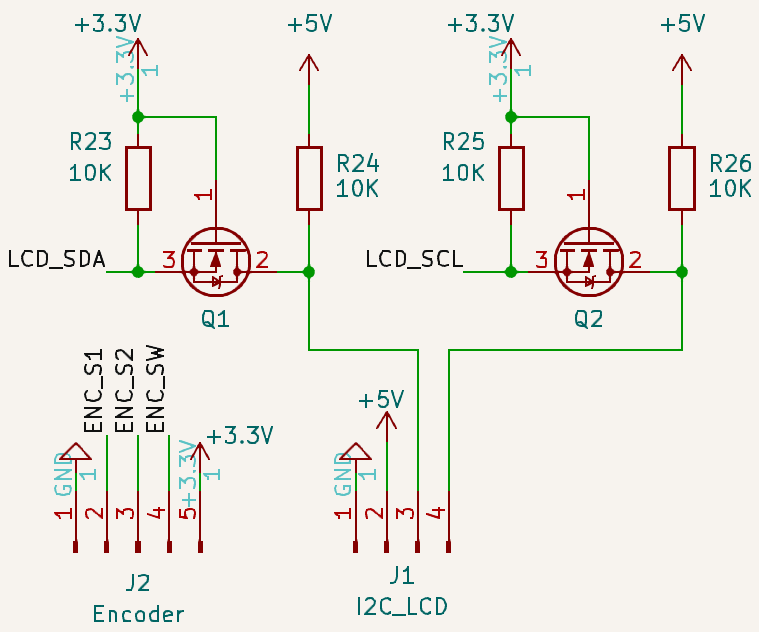
\includegraphics[width=\linewidth]{lcd_schemat.png}
    \caption{Schemat połączeń enkodera oraz wyświetlacza}
    \label{fig:lcd_enc_connection}
\end{figure}

Obsługa modułu enkodera wymaga podłączenia zasilania, sygnałów A i B - wyjść impulsów enkodera oraz sygnału SW - wyjścia przycisku. 
Sygnały A, B oraz SW zostały podłączone bezpośrednio do wyprowadzeń GPIO mikrokontrolera. Obsługa wyświetlacza wymaga podłączenia 
zasilania oraz sygnałów SCL i SDA dla interfejsu I2C używanego do komunikacji z ekspanderem I/O PCF8574 obsługującym wyświetlacz. 
Pierwotnie wyświetlacz oraz ekspander zasilono tak z napięcia 3,3 V. Podczas wstępnego uruchomienia zestawu zauważono, że
obraz na wyświetlaczu jest niewyraźny. Było to spowodowane zbyt niskim napięciem zasilania dla poprawnego funkcjonowania podświetlenia
wyświetlacza. Po zwiększeniu napięcia zasilania do 5 V problem ustąpił. Zmiana wartości napięcia zasilania wymagała zastosowania
konwerterów poziomów logicznych na liniach SCL i SDA, ponieważ mikrokontroler RP2040 pracuje z napięciem 3,3 V. Zastosowany konwerter 
poziomów logicznych jest oparty o tranzystor MOSFET typu N. Ważną właściwością tego typu konwertera jest możliwość konwersja poziomów w obu \
kierunkach która jest w tym wypadku konieczna gdyż linia SDA jest linią dwukierunkową.

\subsubsection{Diody LED oraz przyciski}
Diody LED są sterowane przez trzy rejestry przesuwne 74HC595. Zgodnie z notą aplikacyjną \cite{ti:74hc595}
w celu sterowania układem należy wykonać następujące połączenia:

\begin{itemize}
    \item VCC - zasilanie 3,3 V
    \item GND - masa
    \item SER - linia danych, w pierwszym układzie podłączona do wyprowadzenia GPIO mikrokontrolera natomiast w kolejnych 
    układach podłączona do wyjścia danych  poprzedniego układu
    \item $\overline{SRCLR}$ - linia resetu podłączona na stałe do napięcia zasilania
    \item SRCLK - linia zegara podłączone do GPIO mikrokontrolera
    \item RCLK - linia zegara rejestrów wyjściowych podłączone do GPIO mikrokontrolera
    \item $\overline{OE}$ - włączenie wyjścia podłączone na stałe do masy
\end{itemize}

Na wyjściu układu w stanie wysokim pojawi się napięcie 3,3 volta, zastosowane diody LED charakteryzuje napięcie przewodzenia około 2 V. Charakterystyka
zależności prądu od napięcia diody rośnie bardzo szybko po przekroczeniu napięcia przewodzenia. W celu ograniczenia prądu przepływającego przez diodę
stosujemy szeregowy rezystor. Wartość tego rezystora obliczamy z następującego wzoru: 
\begin{equation}
    R = \frac{V_{CC} - V_{LED}}{I_{LED}} = \frac{3,3 V - 2 V}{10 mA} = 100 \Omega
\end{equation}

\begin{figure}[H]
    \centering
    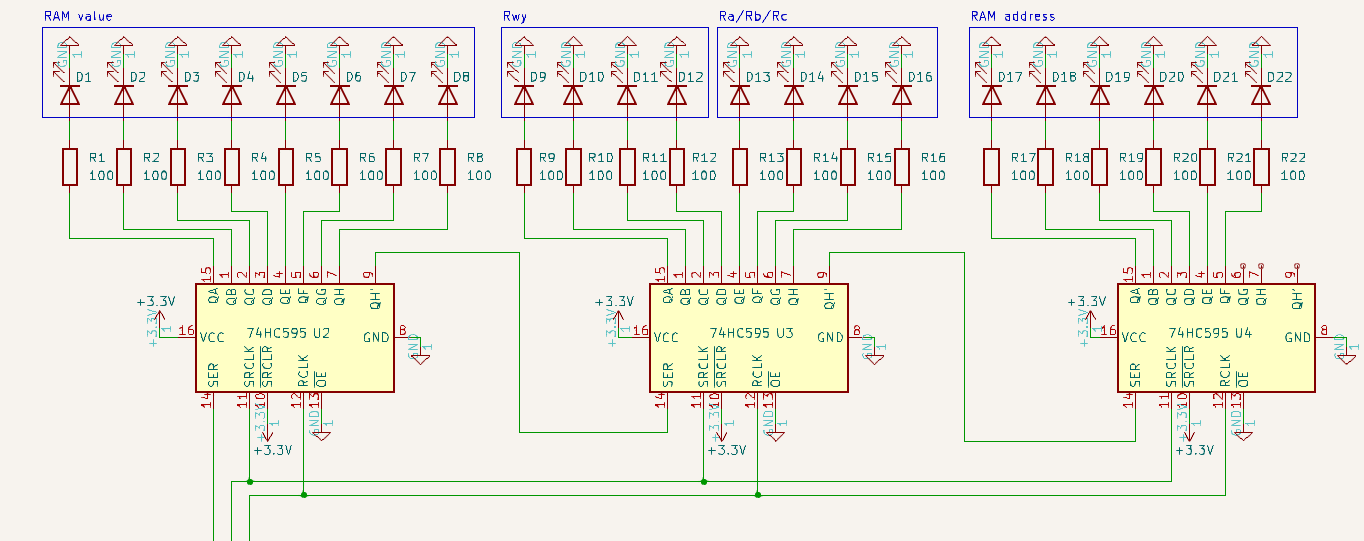
\includegraphics[width=\linewidth]{led_schemat.png}
    \caption{Schemat połączeń rejestrów wraz z diodami LED}
    \label{fig:led_connection}
\end{figure}

Przełączniki zostały podłączone bezpośrednio do wyprowadzeń GPIO mikrokontrolera. Włączenie przycisku powoduje zwarcie linii GPIO z masą
co zostanie odczytane jako stan niski na danym wyprowadzeniu. Stan wysoki w przypadku rozwarcia przycisku jest  wymuszany przez wbudowane
w port wejściowy mikrokontrolera rezystory podciągające do napięcia zasilania.

\begin{figure}[H]
    \centering
    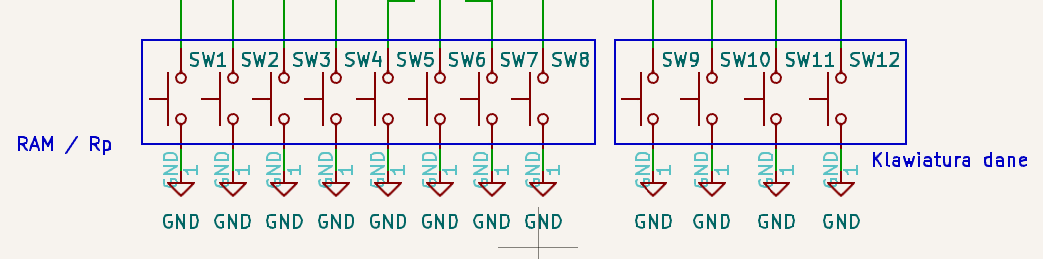
\includegraphics[width=\linewidth]{button_schemat.png}
    \caption{Schemat połączeń przycisków}
    \label{fig:button_connection}
\end{figure}

\subsection{Konstrukcja prototypu}

Poniżej przedstawiono pełen schemat elektryczny zestawu. Na podstawie schematu został wykonany prototyp.

\begin{figure}[H]
    \centering
    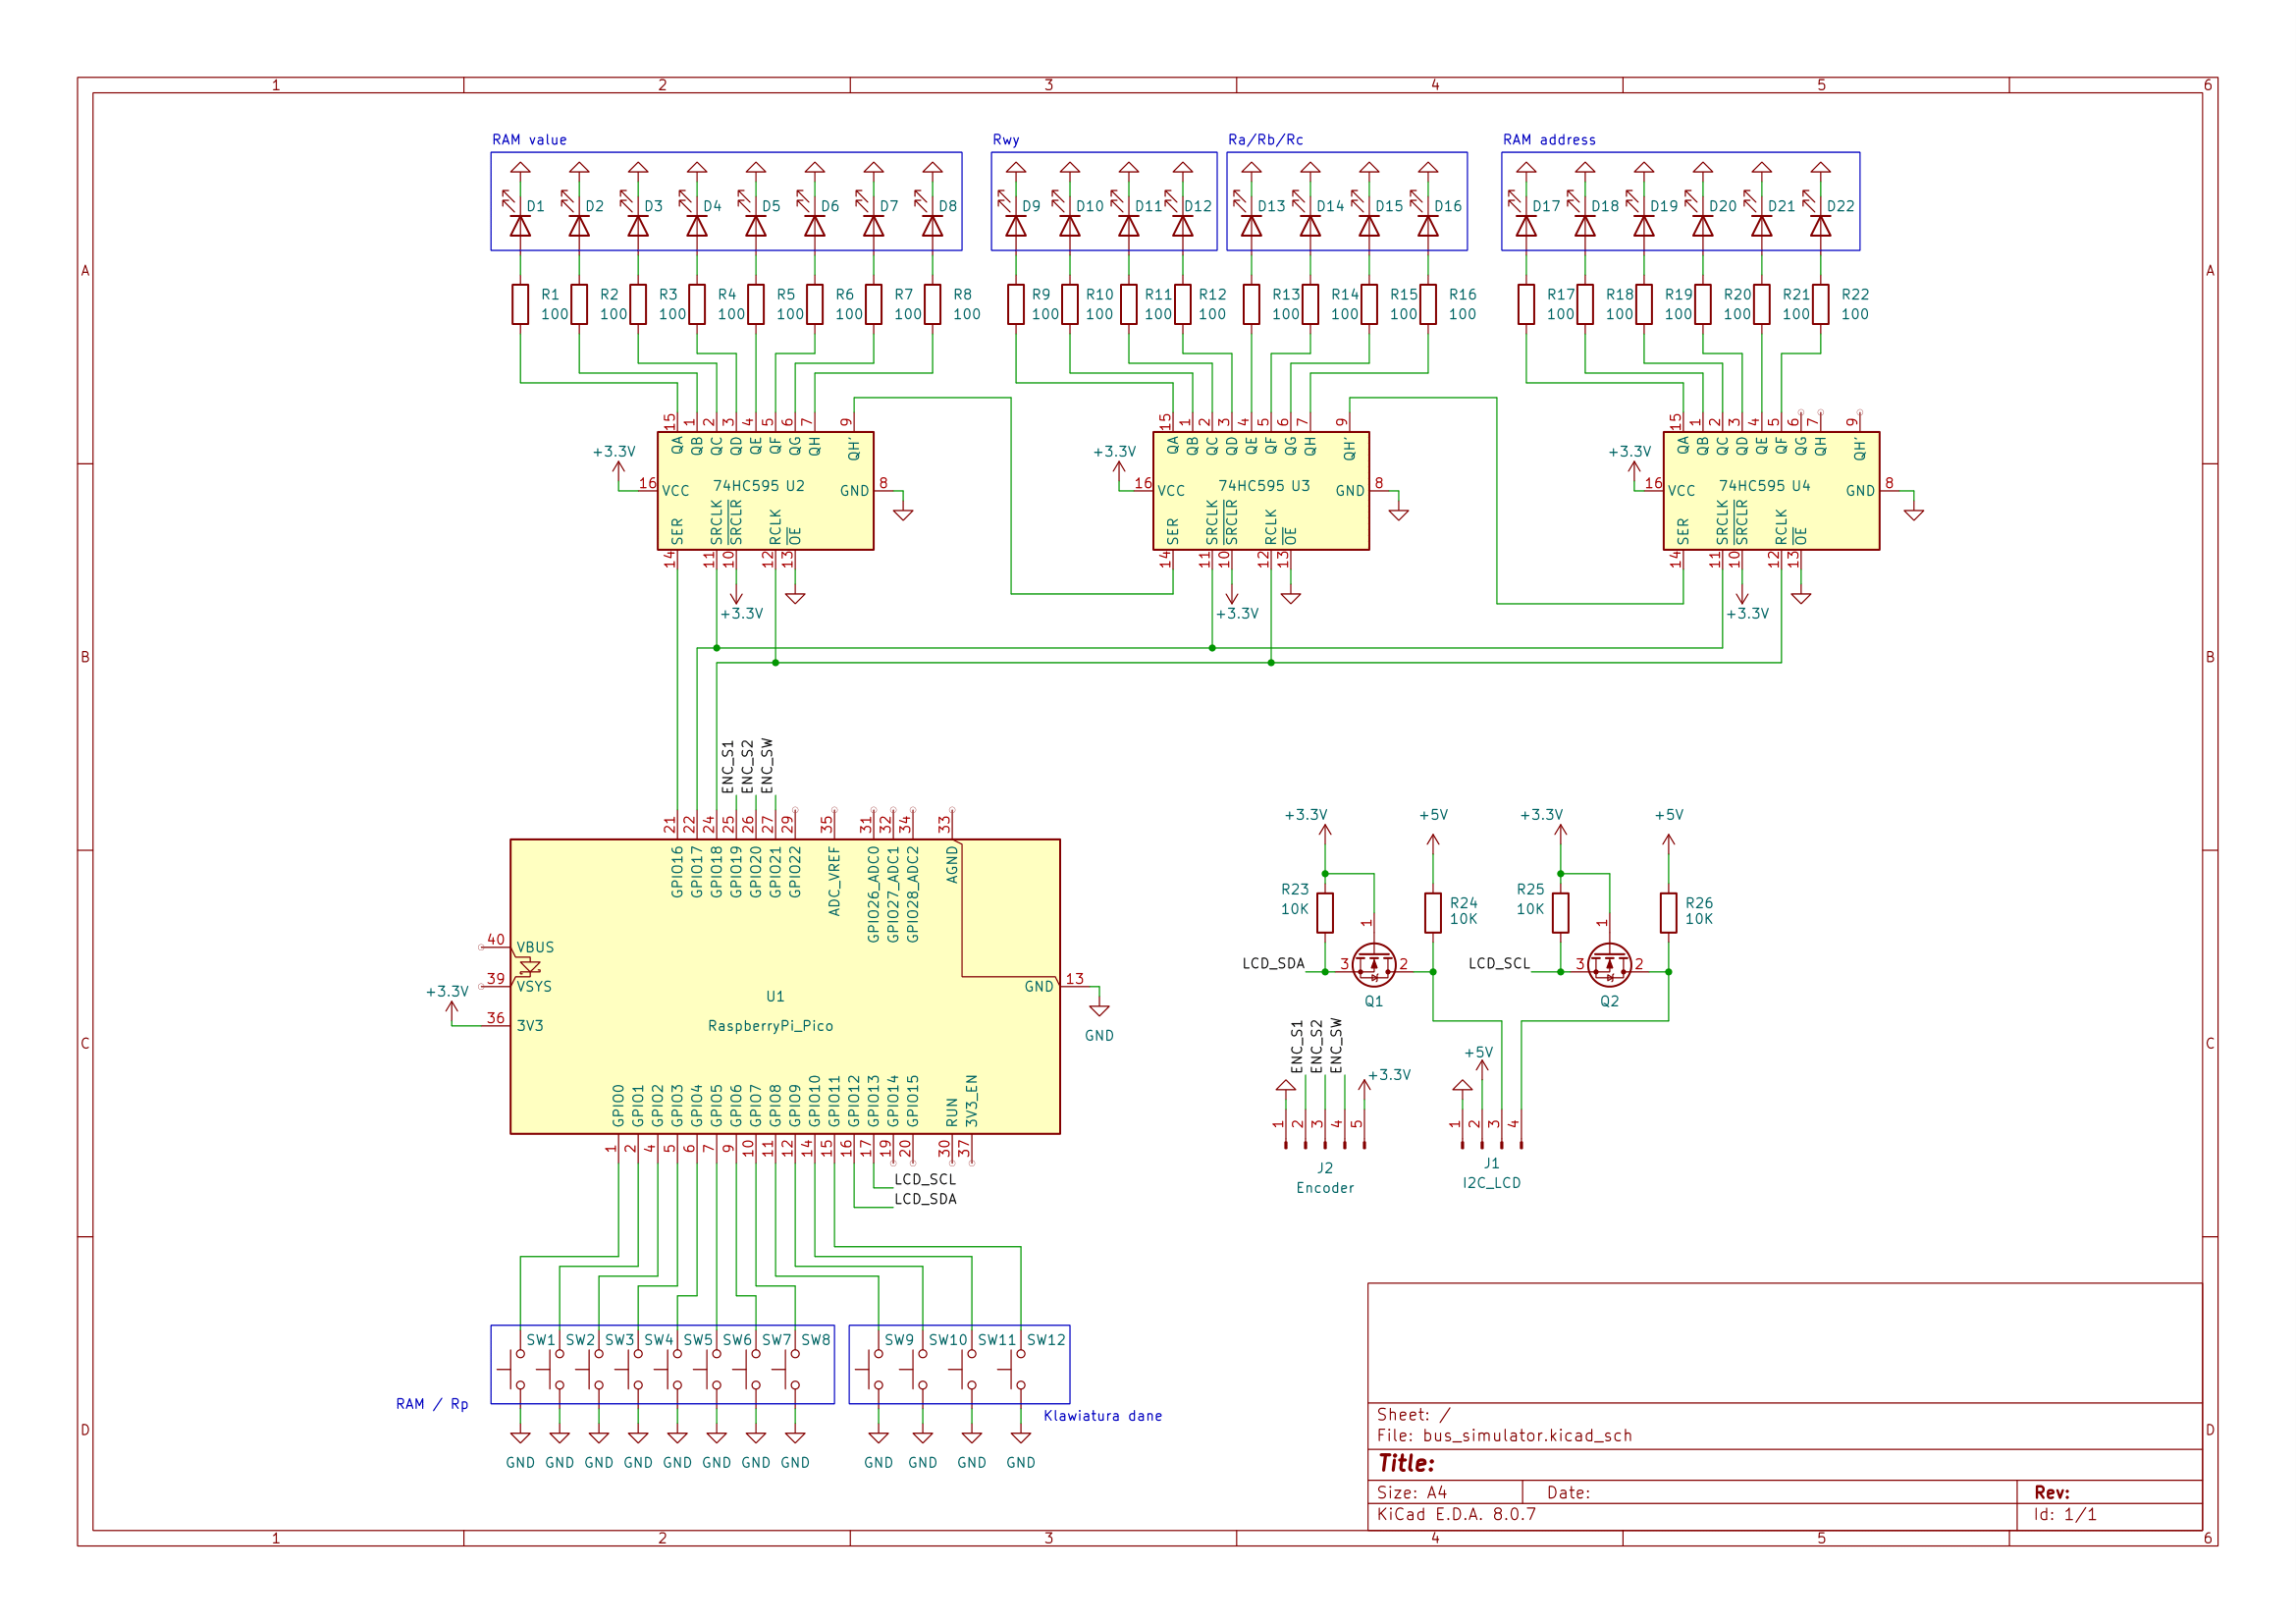
\includegraphics[width=\linewidth]{schemat.png}
    \caption{Schemat elektryczny zestawu}
    \label{fig:electrical_schematic}
\end{figure}

Prototyp został skonstruowany na płytce stykowej. Jest to płytka wykonana z plastiku z otworami w których umieszczane są nóżki elementów lub przewody.
W środku plastikowej konstrukcji znajdują się blaszki które łączą się z elementami wprowadzonymi do otworów. W użytej płytce stykowej cztery sąsiednie
otwory przypadają na jedną blaszkę. Takie rozwiązanie pozwala na szybkie modyfikacje konstruowanego oraz ułatwia testowanie
budowanego układu elektrycznego. Jedną z wad układów na płytkach stykowych są duże pojemności pomiędzy połączeniami wynikające
z konstrukcji płytki. W przypadku budowanego zestawu nie stanowi to problemu gdyż nie występują w nim sygnały o wysokich częstotliwościach.

W konstrukcji wykorzystano trzy połączone ze sobą płytki stykowe. Na pierwszej umieszczono mikrokontroler, przełączniki oraz enkoder.
Na drugiej umieszczono rejestry przesuwne wraz z diodami LED. Na trzeciej umieszczono wyświetlacz LCD wraz z konwerterem poziomów logicznych.

\begin{figure}[H]
    \centering
    \includegraphics[width=\linewidth]{prototype.jpg}
    \caption{Zestaw wykonany na płytce stykowej}    
    \label{fig:prototype}
\end{figure}


\subsection{Część programowa}

\subsubsection{Obsługa diod LED oraz przełączników}

Do obsługi rejestrów przesuwnych oraz przełączników została napisana klasa \texttt{UserIO}. Klasa ta posiada metody ustawiania stanu
diod LED oraz odczytu stanu przełączników. Konstruktor klasy inicjalizuje wyprowadzenia GPIO do których połączone są przyciski jako wejścia oraz
inicjalizuje obiekt \texttt{shift\_register} klasy \texttt{ShiftRegister} który obsługuje rejestry przesuwne. 
\par
Do odczytu przycisków służy metoda \texttt{read\_all\_buttons} która zwraca stan wszystkich przycisków w postaci 16 bitowej liczby.

\begin{lstlisting}[language=C++]
    uint16_t userIO::read_all_buttons(){
    uint16_t button_data = 0;
    for (int i = 0; i < 12; i++){
        button_data |= (digitalRead(buttons[i]) << i);
    }
    return button_data;
}
\end{lstlisting}

Wartość jest odczytywana w pętli wykonywanej dla każdego przycisku. W każdej iteracji odczytywany jest stan danego przycisku który
jest następnie przesuwany o ilość bitów odpowiadającą numerowi przycisku otrzymana wartość poddawana bitowej sumie logicznej z wartością zmiennej
zwracanej przez funkcje. W ten sposób otrzymujemy 16 bitową liczbę w której każdy bit odpowiada stanowi jednego przycisku.
Funkcje \texttt{read\_user\_input\_buttons} oraz \texttt{read\_data\_input\_buttons} odczytują odpowiednio dane
z klawiatury wprowadzania danych na szynę oraz z klawiatury wprowadzania danych do RAM/$R_P$. Obydwie funkcje używają funkcji \texttt{read\_all\_buttons}
do odczytu stanu przycisków a następnie wydobywają z odczytanej wartości odpowiednie bajty danych.
\par
Obsługa diod LED odbywa się za pomocą metody \texttt{render\_led}. 

\begin{lstlisting}[language=C++]
    void userIO::render_led(const bus_cpu_status status){
        uint8_t led_values[REG_NO] = {0, 0, 0};
        led_values[0] = status.RAM_value;
        led_values[1] = status.Rwy;
        switch (displayed_register){
            case Ra:
                led_values[1] |= (status.Ra << 4);
                break;
            case Rb:
                led_values[1] |= (status.Rb << 4);
                break;
            case Rc:
                led_values[1] |= (status.Rc << 4);
                break;
            default:
                led_values[1] |= (status.Ra << 4);
                break;
        }
        led_values[2] = status.RAM_address;
        shift_register.setAll(led_values);
    }
\end{lstlisting}

Funkcja ta przyjmuje jako argument strukturę \texttt{bus\_cpu\_status} która zawiera wartości rejestrów, słowa pamięci RAM oraz adresu pamięci RAM.
Przekazane wartości są przypisywane do tablicy w odpowiedniej kolejności tak aby wyświetliły się na odpowiednich diodach LED. W tej funkcji
realizowane jest również przełączanie wyświetlanych rejestrów. W zależności od wartości zmiennej \texttt{displayed\_register} na diodach LED
wyświetlana jest wartość odpowiedniego rejestru. Na koniec wartości z tablicy są przekazywane do metody \texttt{setAll} obiektu \texttt{shift\_register}
która ustawia wartości w rejestrach przesuwnych.

\subsubsection{Symulacja jednostki arytmetyczno-logicznej}

Symulacja jednostki arytmetyczno-logicznej została zrealizowana w klasie \texttt{ALU}.
Klasa ta posiada metody realizujące zadaną operacje oraz ustawiania kodu operacji. Metoda \texttt{set\_opcode} ustawia kod operacji.
W celu poprawnego ustawienia kodu powinna ona zostać wywołana trzy razy.

\begin{lstlisting}[language=C++]
    void alu::set_opcode(const uint8_t _opcode){
        if(opcode_set_count == 2){
            opcode = opcode << 1;
            opcode |= _opcode;
            opcode_set_count = 0;
        }
        else{
            opcode = opcode << 2;
            opcode |= _opcode;
        }
        opcode_set_count++;
    }
\end{lstlisting}

Podczas pierwszych dwóch wywołań metoda kod operacji jest przesuwany o dwa bity w lewo, a następnie do dwóch najmłodszych bitów zostają
zapisane dwa najmłodsze bity kodu przekazanego jako argument funkcji. W trzecim wywołaniu funkcji kod operacji jest przesuwany o jeden bit w lewo,
a następnie do najmłodszego bitu zostaje przepisana wartość najmłodszego bitu kodu przekazanego do argumentu funkcji. W ten sposób uzyskujemy
pełen pięciobitowy kod operacji. 
\par
Metoda \texttt{calculate} oblicza wynik operacji zadanej kodem operacji. Jako argumenty funkcja przyjmuje dwie liczby na których ma zostać wykonana
operacja. Funkcja na początku rozpatruje najstarszy bit kodu operacji. W zależności od jego wartości wykonana zostanie operacja logiczna lub arytmetyczna.
Następnie funkcja wykonuje odpowiednią operacje zależnie od pozostałych czterech bitów kodu operacji. Ze względu na 4 bitową architekturę zestawu oraz
brak implementacji bitu przeniesienia w oryginalnym zestawie funkcja zwraca tylko cztery najmłodsze bity wyniku operacji. 

\subsubsection{Symulacja pozostałych elementów zestawu}

Symulacja pozostałych elementów zestawu została zrealizowana w klasie \texttt{CPU}. Klasa ta implementuje funkcje symulujące działanie zestawu oraz
szereg funkcji pomocniczych służących do sterowania pracą zestawu, ustawiania jego parametrów czy odczytu jego stanu.
W klasie tej jako zmienne prywatne zdefiniowane są wszystkie rejestry wchodzące w skład zestawu.

\begin{lstlisting}[language=C++]
    class bus_cpu{
        private:
            uint8_t Ra;
            uint8_t Rb;
            uint8_t Rc;
            uint8_t Rwy;
            uint8_t R1;
            uint8_t R2;
            uint8_t Ri;
            uint8_t Ri_tmp;
            uint8_t Gs;
        
            uint8_t Rp_address;
        
            std::array<uint8_t, RAM_SIZE> RAM;
            std::array<uint8_t, PROGRAM_SIZE> Rp;
        
            alu ALU;
\end{lstlisting}

Pomimo, że rejestry są czterobitowe zostały zdefiniowane jako ośmiobitowe liczby całkowite bez znaku. Jest to spowodowane tym, że w języku C++ nie 
ma typów danych o mniejszej niż 8 liczbie bitów. Zdefiniowano także pamięć RAM oraz rejestr $R_P$ jako tablice o odpowiednich rozmiarach. 
Klasa posiada również obiekt klasy \texttt{ALU} symulującej jednostkę arytmetyczno-logiczną.
\par
Podstawową funkcją klasy jest funkcja \texttt{process\_microcycle} która realizuje wykonuje jeden mikrocykl. 
W pierwszej kolejności na podstawie wartości rejestru $R_I$ oraz wartości generatora stanów $G_S$ obliczany jest adres w pamięci RAM z którego 
odczytana zostanie instrukcja Następnie z odczytanej instrukcji wydobywane są bity operacji dla ALU, kod transmitera oraz odbiornika. 

\begin{lstlisting}[language=C++]
    ucycle_status bus_cpu::process_microcycle(){
    uint8_t address = calculate_address();
    uint8_t instruction = RAM[address]; 
    uint8_t alu_opcode = instruction & 0b00000011;
    uint8_t rx_ctrl = (instruction & 0b00011100) >> 2;
    uint8_t tx_ctrl = (instruction & 0b11100000) >> 5;
    uint8_t* transmiter;
    uint8_t* receiver;
    uint8_t alu_result = 0;
\end{lstlisting}
\par
Symulacja transmisji danych na szynie odbywa się na zasadzie wskaźników. W zależności od wartości kodu transmitera oraz odbiornika do
wskaźników \texttt{transmiter} oraz \texttt{receiver} przypisywane są odpowiednie adresy odpowiednich zmiennych reprezentujących odbiorniki oraz nadajniki.
W przypadku gdy odbiornikiem jest $R_I$, $R_1$ lub $R_2$ dodatkowo ustawiany jest kod operacji dla ALU. 
Na koniec wskaźniki wartość pod adresem transmitera jest przypisywana pod adres odbiornika.
\par
W przypadku gdy nadajnikiem jest klawiatura wprowadzania danych na szynę funkcja zwraca kod \texttt{NEED\_INPUT} który jest interpretowany
przez maszynę stanów sterującą wykonaniem programu. Kiedy dane zostaną pobrane przez użytkownika ustawiona zostaje flaga \texttt{user\_input\_ready}
która powoduje poprawne wykonanie transmisji przy kolejnym wywołaniu funkcji przetwarzania mikrocyklu.

\begin{lstlisting}[language=C++]
        case 5: 
            if(!user_input_ready){
                return NEED_INPUT;
            }
            transmiter = &user_input;
            user_input_ready = false;
            break;
\end{lstlisting}
\par
Kiedy funkcja zakończy przetwarzanie mikrocyklu wartość generatora GS jest inkrementowana. Jeżeli wartość generatora przekroczy wartość 3
zwiększany jest adres rejestru $R_P$ a generator jest resetowany. Wartość zmiennej R\_I jest ustawiana na wartość zmiennej R\_I\_tmp.
Wartość rejestru $R_I$ musi pozostać stała przez okres trwania cyklu (4 mikrocykle) ponieważ jest ona używana do obliczenia adresu pamięci RAM
z którego odczytywana jest instrukcja. Po przepełnieniu się generatora GS można zmienić wartość w rejestrze $R_I$.
 
\begin{lstlisting}[language=C++]
    Gs++;
    if(Gs > 3){
        Rp_address++;
        Gs = 0;
        ALU.clear_opcode();
        Ri = Ri_tmp;
    }
    return SUCCESS;
}
\end{lstlisting}

\par
Funkcja \texttt{schedule\_execution} jest funkcją sterującą pracą zestawu. Funkcja ta jest wywoływana w głównej pętli programu. 
Kontrola pracy zestawu odbywa się za pomocą maszyny stanów:

\begin{itemize}
    \item \texttt{EXECUTION} - zestaw wykonuje mikrocykl
    \item \texttt{CYCLE\_DONE} - zakończyło się wykonywanie cyklu lub mikrocyklu
    \item \texttt{USER\_INPUT} - zestaw oczekuje na wprowadzenie danych przez użytkownika
    \item \texttt{DONE} - zestaw zakończył pracę
    \item \texttt{READY} - zestaw jest gotowy do rozpoczęcia pracy
    \item \texttt{EXCEPTION} - wystąpił błąd
\end{itemize}

\par
Kiedy zestaw jest w stanie \texttt{EXECUTION} funkcja wywołuje funkcję \texttt{process\_microcycle} która wykonuje mikrocykl.
W przypadku pracy w trybie Program funkcja implementuje dodatkowy mechanizm opóźniający wykonywanie kolejnych mikrocykli.
Jest to konieczne ze względu na dużą prędkość mikrokontrolera która powoduje że zmiany stanów na diodach LED wizualizujących pracę 
zestawu są zbyt szybkie.

\begin{lstlisting}[language=C++]
    if (internal_state == EXECUTION){
            uint64_t time_difference = millis() - last_successful_ucycle;
            if(time_difference > execution_speed || type == CYCLE || type == MICRO_CYCLE){
                ucycle_return = process_microcycle();
            }
\end{lstlisting}

\par
Następnie przetwarzana jest wartość zwracana przez funkcję \texttt{process\_microcycle}. W przypadku gdy funkcja zwróciła kod \texttt{SUCCESS}
dla trybów pracy Cykl oraz Mikrocykl sprawdzane są warunki zakończenia cyklu pracy zestawu. Następnie jest sprawdzany warunek zakończenia pracy
zestawu niezależnie od trybu pracy. W przypadku zestaw wykonał wszystkie instrukcje znajdujące się w rejestrze $R_P$ zestaw przechodzi w stan \texttt{DONE}.

\begin{lstlisting}[language=C++]
            switch (ucycle_return){
                case SUCCESS:
                last_successful_ucycle = millis();
                    switch (type){
                        case CYCLE:
                            if(Gs == 0){
                                internal_state = CYCLE_DONE;
                            }
                            break;
                        case MICRO_CYCLE:
                            internal_state = CYCLE_DONE;
                            break;
                        case PROGRAM:
                            break;
                        default:
                            internal_state = EXCEPTION;
                            break;
                    }
                    if (Rp_address > 15){
                        internal_state = DONE;
                    }
                    break;
                case NEED_INPUT:
                    internal_state = USER_INPUT;
                    break;
                case ERROR:
                    internal_state = EXCEPTION;
                    break;
                default:
                    internal_state = EXCEPTION;
                    break;
            }
        }
        return internal_state;
    }
\end{lstlisting}

\par
W przypadku gdy funkcja zwróciła kod \texttt{NEED\_INPUT} zestaw przechodzi w stan \texttt{USER\_INPUT}. W tym stanie zestaw oczekuje na wprowadzenie
wartości przez użytkownika. Po wprowadzeniu wartości zestaw przechodzi w stan \texttt{EXECUTION} i kontynuuje pracę. W przypadku wystąpienia
błędu zestaw przechodzi w stan \texttt{EXCEPTION}. Na koniec funkcja zwraca stan Wewnętrznej maszyny stanów.

\subsubsection{Obsługa interfejsu użytkownika}

W celu obsługi interfejsu użytkownika przy pomocy biblioteki Arduino menu w pierwszej kolejności należy zdefiniować sterowniki urządzeń
wejściowych oraz wyjściowych. W naszym przypadku urządzeniami wejściowymi jest obrót enkoderem oraz wbudowany w enkoder przycisk, urządzeniem wyjściowym
jest wyświetlacz LCD. Biblioteka Arduino menu dostarcza sterowniki enkodera oraz przycisku w formie klas.

\begin{lstlisting}[language=C++]
    encoderIn<ENC_S2,ENC_S1> encoder;//simple quad encoder driver
    encoderInStream<ENC_S2,ENC_S1> encStream(encoder,ENC_SENSITIVITY);

    //a keyboard with only one key as the encoder button
    keyMap encBtn_map[]={{-ENC_SW,defaultNavCodes[enterCmd].ch}};
    keyIn<1> encButton(encBtn_map);//1 is the number of keys

    //input from the encoder + encoder button + serial
    menuIn* inputsList[]={&encStream,&encButton};
    chainStream<2> in(inputsList);//2 is the number of inputs
\end{lstlisting}

Urządzenia wejściowe obsługiwane są na zasadzie strumieni. W powyższym kodzie zdefiniowano strumień wejściowy \texttt{chainStream} który
jest połączeniem strumieni enkodera oraz przycisku.
\par
Obsługa strumienia wyjściowego dla wyświetlacza LCD wymaga zadeklarowania obiektu klasy \texttt{LiquidCrystal\_PCF8574} oraz przy
pomocy makra \texttt{MENU\_OUTPUTS} dostarczanego przez bibliotekę Arduino menu przekazania obiektu do listy wyjść dla menu.

\begin{lstlisting}[language=C++]
    LiquidCrystal_PCF8574 lcd(0x27);
    MENU_OUTPUTS(out, 3, LCD_OUT(lcd,{0,0,20,4}), NONE);
\end{lstlisting}

\par
Następnym krokiem jest deklaracja głównego okna menu. Jest to pierwsze okno które jest wyświetlane po uruchomieniu programu.
Tworzenie okna menu odbywa się przy pomocy makra \texttt{MENU}. Makro to przyjmuje szereg argumentów które decydują o 
tytule, wyglądzie, oraz reakcjach okna na zdarzenia. Jako argumenty przekazywane są również opcje które będą dostępne w oknie.
Okno jest ustawiane jako główne przy pomocy makra \texttt{NAVROOT}.

\begin{lstlisting}[language=C++]
    MENU(busMainMenu,"Szyna danych",doNothing,noEvent,wrapStyle
    ,SUBMENU(start_execution)
    ,SUBMENU(ram_edit)
    ,SUBMENU(program_edit)
    ,FIELD(execution_clock,"Zegar","Hz",1,20,1,0,set_exec_speed_commit,anyEvent,wrapStyle)
    ,OP("Reset",reset_system_commit,enterEvent)
  );
  NAVROOT(nav, busMainMenu, 3, in, out);
\end{lstlisting}

\par
Biblioteka Arduino menu posiada szereg wbudowanych typów opcji które można wykorzystać w oknach menu. W projekcie wykorzystano
następujące opcje:
\begin{itemize}
    \item \texttt{SUBMENU} - opcja która przenosi do innego okna
    \item \texttt{FIELD} - pozwala na edycję wartości oraz wyświetlanie wartości zmiennej
    \item \texttt{OP} - pole tekstowe które może reagować na zdarzenia takie jak wciśnięcie przycisku
    \item \texttt{EXIT} - powrót do poprzedniego okna
\end{itemize}

\par
Obsługa opcji \texttt{FIELD} wymaga zdefiniowania zmiennej w której będzie przechowana zmieniana wartość oraz granic jakie wartość może przyjąć.
W przykład opcji o nazwie \texttt{"Zegar"} znajdującej się na głównym ekranie zmienna \texttt{execution\_clock} przechowuje wartość zegara,
minimalna wartość to 1, maksymalna 20, a krok zmiany to 1. Dodatkowo zdefiniowano funkcje \texttt{set\_exec\_speed\_commit} która jest wywoływana
podczas zmian wartości zmiennej. Funkcja ta na bieżąco przekazuje wartość zmiennej do obiektu klasy odpowiedzialnej za symulację pracy zestawu.

\begin{lstlisting}[language=C++]
    uint8_t execution_clock = 10;

    result set_exec_speed_commit(eventMask e,navNode& nav, prompt &item) {
      cpu.set_execution_speed(1000/execution_clock);
      return proceed;
    }
\end{lstlisting}

\par
Obsługa opcji \texttt{OP} polega na zdefiniowaniu funkcji która zostaje wywołana po wciśnięciu przycisku. W przypadku opcji \texttt{"Reset"}
znajdującej się na głównym ekranie wywoływana jest funkcja \texttt{reset\_system\_commit} która resetuje stan zestawu.

\begin{lstlisting}[language=C++]
    result reset_system_commit(eventMask e,navNode& nav, prompt &item) {
        cpu.clear();
        return proceed;
      }
\end{lstlisting}

\par
Zapis wartości do pamięcią RAM oraz $R_P$ odbywa się na podobnej zasadzie. Zadeklarowano zmienne \texttt{ram\_address\_edit} oraz \texttt{ram\_value}
przechowujące obecną wartość adresu pamięci RAM oraz wartość w obecnej komórce pamięci RAM. Obydwie te zmienne są przypisywane
do odpowiednich opcji \texttt{FIELD} w oknie edycji pamięci RAM.

\begin{lstlisting}[language=C++]
    uint8_t ram_address_edit = 0;
    uint8_t ram_value = 0;
    
    MENU(ram_edit,"Zapis RAM",doNothing,noEvent,noStyle
      ,FIELD(ram_address_edit,"Adres:","",0,63,1,0,display_ram,anyEvent,wrapStyle)
      ,OP("Zapisz",edit_ram_commit,enterEvent)
      ,FIELD(ram_value,"Wartosc:","",0,255,0,0,doNothing,noEvent,noStyle)
      ,EXIT("<Wroc")
    );
    
\end{lstlisting}

Po wybraniu odpowiedniego adresu w opcji \texttt{"Adres"} należy wcisnąć opcję \texttt{"Zapisz"} która wywoła funkcję \texttt{edit\_ram\_commit}.
Funkcja ta zapisuje wartość z klawiatury wprowadzania danych do pamięci RAM na adresie \texttt{ram\_address\_edit}. Oraz inkrementuje wartość
w zmiennej przechowującej adres.

\begin{lstlisting}[language=C++]
    result edit_ram_commit(eventMask e,navNode& nav, prompt &item) {
        cpu.set_RAM(ram_address_edit, io.read_data_input_buttons());
        ram_address_edit++;
        ram_value = cpu.get_RAM(ram_address_edit);
        return proceed;
      }
\end{lstlisting}

W celu zapewnienia interaktywnego podglądu wartości pamięci RAM pod aktualnie wybranym adresem do opcji \texttt{"Adres"} przypisano 
funkcję \texttt{display\_ram} wywoływaną przy każdym zdarzeniu. Powoduje to wywołanie funkcji przy każdej zmianie adresu w polu edycji.
Funkcja ta pobiera wartość z pamięci RAM pod adresem \texttt{ram\_address\_edit} i przypisuje ją do zmiennej \texttt{ram\_value} 
co powoduje aktualizacje wartości wyświetlanej w polu \texttt{"Wartość"}.

\begin{lstlisting}[language=C++]
      result display_ram(eventMask e,navNode& nav, prompt &item) {
        ram_value = cpu.get_RAM(ram_address_edit);
        return proceed;
      }
\end{lstlisting}

\par
Ekran pobierania danych od użytkownika został zrealizowany w funkcji \texttt{user\_input}. Funkcja ta jest wywoływana w momencie gdy zestaw
oczekuje na dane od użytkownika. Funkcja wyświetla komunikat proszący o podanie wartości. Po wciśnięciu przycisku pobiera wartość z klawiatury.

\begin{lstlisting}[language=C++]
    result user_input(menuOut& o,idleEvent e) {
        switch(e) {
          case idleStart:
            o.print("Wprowadz wartosc");
            break;
          case idleEnd:
            cpu.take_user_input(io.read_user_input_buttons());
          break;
        }
        return proceed;
      }
\end{lstlisting}

\subsubsection{Główna pętla programu}

Program rozpoczyna się od wywołania funkcji \texttt{setup}. W tej funkcji przeprowadzana jest inicjalizacja wyświetlacza LCD, enkodera
oraz obiektu nawigacyjnego biblioteki Arduino Menu. Następnie wywoływana jest funkcja \texttt{loop} w której znajduje się główna logika programu.
Funkcja ta jest wywoływana w nieskończonej pętli.

\begin{lstlisting}[language=C++]
    void loop() {
        bus_cpu_state cpu_state;
        nav.poll();
        cpu_state = cpu.schedule_execution();
      
        if{cpu_state == bus_cpu_state::USER_INPUT} {
          nav.idleOn(user_input);
        }
        else if{cpu_state == bus_cpu_state::EXCEPTION} {
          Serial.println("Zestaw napotkal blad"); 
        }
      
        io.set_displayed_register(displayed_register);
        cpu.get_register_values(cpu_status);
        io.render_led(cpu_status);
        delay(50);
      }
\end{lstlisting}

W głównej pętli programu jest wywoływana funkcja \texttt{poll} obiektu nawigacyjnego. Funkcja ta odpowiada za przetwarzanie zdarzeń
związanych z interfejsem użytkownika. Następnie wywoływana jest funkcja \texttt{schedule\_execution} która zarządza pracą symulatora
szyny danych. W zależności od zwróconego stanu zestawu wywoływane są odpowiednie funkcje. W przypadku gdy zestaw oczekuje na dane od użytkownika
wywoływana jest funkcja \texttt{idleOn} która wywoła okno menu odpowiedzialne za wprowadzanie danych. W przypadku wystąpienia błędu zostanie
wydrukowana informacja na porcie szeregowym. Kolejne trzy funkcje odpowiadają za aktualizacje stanu diod LED na podstawie aktualnych wartości
rejestrów zestawu. Na końcu pętli programu znajduje się opóźnienie 50 milisekund które zapewnia stabilne działanie programu.

\end{document}